\documentclass[12pt]{article}
\usepackage[english]{babel}
\usepackage{float}
\usepackage[utf8]{inputenc}
\usepackage{graphicx}
\usepackage{mathtools}
\usepackage[nottoc]{tocbibind}
\usepackage{tikz}
\usepackage{verbatim}
\usepackage{setspace}
\usepackage{xcolor}
\usepackage{sectsty}
\usepackage[tableposition = top]{caption}


\definecolor{melisa}{RGB}{180,120,20}
\definecolor{hakan}{RGB}{180,0,20}
\definecolor{ugur}{RGB}{120,0,50}

\sectionfont{\color{melisa}}
\subsectionfont{\color{hakan}}
\subsubsectionfont{\color{esra}}

\setstretch{1.5}

\usepackage{geometry}
 \geometry{
 a4paper,
 total={170mm,257mm},
 left=25mm,
 top=25mm,
 right=25mm,
 bottom=25mm,
 }

\begin{document}


\begin{titlepage}
	\centering

	{\scshape\LARGE Middle East Technical University \par}
	\vspace{0.2cm}
	{\scshape\LARGE EE464 Power Electronics  \par}
	\vspace{3cm}

    
\includegraphics{fiero-logo.png}\par
    {\scshape\LARGE\textit{\textbf{"Turning Coffee into Electricity"}}   \par}
    \vspace{3 cm}
	
	
	{\scshape\LARGE Project 2 Report \par}
	\vspace{1 cm}
	{\Large\itshape \today \par}
		\vspace{0.3 cm}



	
	{\Large\itshape Asena Melisa SARICI -2031284\par}
	\vspace{0.1cm}

	{\Large\itshape Hakan POLAT -\par}
	\vspace{0.1cm}
	
	{\Large\itshape Uğur Can YILMAZ - 2031680  \par}
	\vspace{0.1cm}
	
	
	To be submitted to\par
	{\Large\itshape{Ozan \textsc{KEYSAN}\par}}
	
	

\end{titlepage}


\tableofcontents
\newpage

\newpage
\section{Introduction}

As Fiero Converters, we manufacture 230 V AC to 9 V DC, 10 W Flyback  Converters. This documents shows the detailed pre-manufacturing process of designing, simulating of the converter and the controller of the product. The design to be used in the simulations is provided in figure \ref{fig:design}.



\section{Design Procedure}
Throughout the design procedure we followed the steps of Wurth Transformers.\\
We started our design by defining our specs for the flyback converter which is present in \ref{tab:spec}.
\begin{table}[H]
\centering

\label{tab:spec}
\begin{tabular}{|l|l|}
\hline
$V_{in} $ & $220 V_{ac}$ \\ \hline
$V_{out}$ & 9 V           \\ \hline
$P_{out}$ & 9 W           \\ \hline
\end{tabular}
\caption{Specs of our flyback converter design}
\end{table}


The flyback converter transfers the power stored in the core in off state and the $\Delta I_{lm}$ stays the same since its formula depends on constant values.
\begin{equation*}
    \Delta I_{lm}= \dfrac{V_{in}DT_{s}}{L_{m}}
\end{equation*}
Therefore it is important to let the core have enough discharge time to avoid saturation. Taking these limitations into concideration we decided $D_{max}=0.4$ for the design of the converter.\\
Next step the determination of $V_{in}$ and $V_{out}$. We plan on rectifying the AC voltage to DC using a full bridge diode rectifier and generate a DC voltage using a DC-link capacitor. According to our calculations the $V_{in,dc}$ varies between 300-325 V. As for the $V_{out}$ we will design it for a $V_{out}$ of 10.5 V which also takes the voltage drop in the diode.\\
Knowing $D_{max}$,$V_{in}$ and $V_{out}$ we can calculate the approximate turns ratio using the formula below.
\begin{equation*}
    \dfrac{N1}{N2}=\dfrac{D_{max}}{1-D_{max}}\dfrac{V_{in,min}}{V_{out}}= 19 
\end{equation*}
By recalculating the $D_{max}$ we obtain;

\begin{equation*}
    D_{max}=\dfrac{19}{12+\dfrac{300}{10.5}}=0.399 
\end{equation*}
The next step is to choose the voltage and current rating of the switch. We are using a mosfet since it has a faster switching response and the current on the primary side during on time is low.\\
During off state the $V_{out}$ induces voltage on the primary winding which is $V_{primary}=-V_{d}$.
Therefore the blocking voltage is $V_{switch}=2*V_{in,max}$.
Also a safety margin for the switching peak voltages results in

\begin{equation*}
    V_{sw,max}=2 V_{in,max}+ V_{in,max}=3V_{in,max}=844 V
\end{equation*}
The current rating can be calculated from

\begin{equation*}
    I_{rated,sw}=\dfrac{P_{out}}{V_{out}}*\dfrac{N2}{N1}=0.05A
\end{equation*}
Also in this case a safety margin will be added.\\
The next step is the calculation of the $L_{lm}$ which results in a \%25 ripple in $I_{out}$(Our starting assumption is \%25) 
. Again by using the $\Delta I_{lm}$ equation (this time for off state),

\begin{equation*}
    L_{sekondary}=\dfrac{V_{out}(1-D_{max})}{0.25I_{avg,seconcary}frequency}=\dfrac{10.5(1-0.4)}{0.25*2*62500}=201.6 \mu H
\end{equation*}
If we reflect the found $L_{secondary}$ to primary we get
$L_{primary}=72mH$. \\
After calculating the core inductance we should now consider the $A_{e}$ and $B_{sat}$ of our core. Since the equation
\begin{equation*}
   N_{primary}>\dfrac{L_{primary}I_{primary,max}}{B_{sat}A_{e}}
\end{equation*}
must hold.\\
Our core has an $A_{e}=125mm^2$ and $B_{sat}=0.3T$ by inserting the values to the equation we obtain,
\begin{equation*}
   N_{primary}> 224.64
\end{equation*}
For calculation simplicity and to make the $N_{primary}$
an interger value we selected,
\begin{equation*}
   N_{primary}= 228
\end{equation*}
\begin{equation*}
   N_{secondary}= 12
\end{equation*}
After selecting the turns ratios we should select proper commercial cables. By checking the rated currents, fill factor and our core area we choose the cable types AWG28 and AWG21 for primary and secondary side respectively.



\section{Isolated Converter Simulation}

The design is made using \cite{}. There is snubber in order to reduce the current and voltage stress the MOSFET endures during operation. The resultant effect of the snubber is clearly observed in the simulations as well. The simulations were done synchronously with the implementation and hence the design parameters for the switch, diode and the transformer are taken from the implemented products.

\begin{figure}[H]
    \centering
    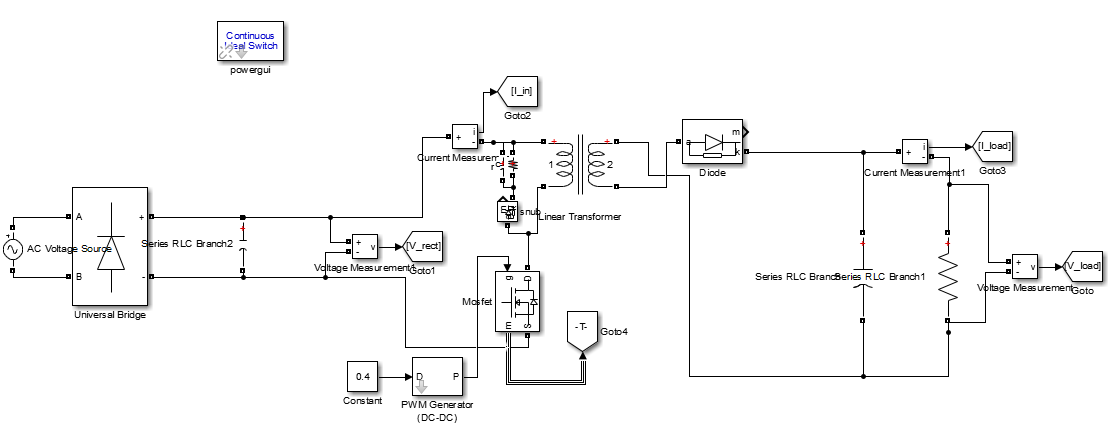
\includegraphics[width=15 cm]{Design}
    \caption{Flyback Design}
    \label{fig:design}
\end{figure}

\subsection{Part I. Steady State Operation of the Converter}

The figures \ref{fig:loadvoltage}, \ref{fig:loadcurrent}, \ref{fig:rectifier}, \ref{fig:display} show the simulation waveforms and the resultant voltage, current and power outputs for the calculated values of maximum duty cycle, turns ratio, reasonable capacitor values and resistance for the ideal case.



\begin{figure}[H]
    \centering
    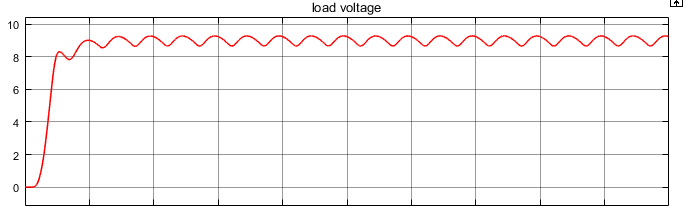
\includegraphics[width=15 cm]{LoadVoltage}
    \caption{Load Steady State Voltage}
    \label{fig:loadvoltage}
\end{figure}

\begin{figure}[H]
    \centering
    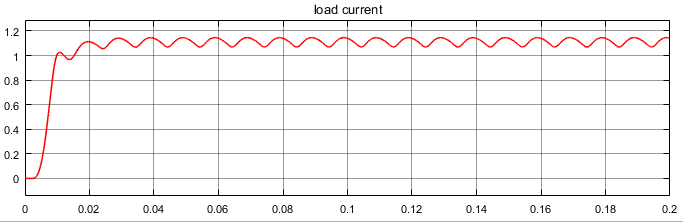
\includegraphics[width=15 cm]{LoadCurrent}
    \caption{Load Steady State Current}
    \label{fig:loadcurrent}
\end{figure}

\begin{figure}[H]
    \centering
    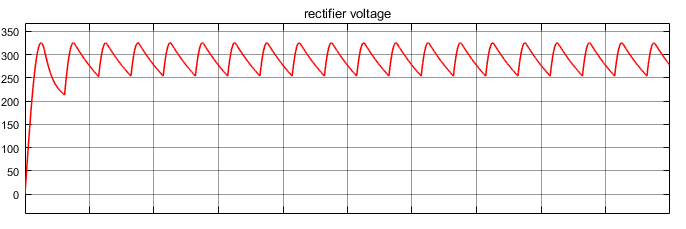
\includegraphics[width=15 cm]{RectifieVoltage}
    \caption{Rectifier Output Voltage at Steady State}
    \label{fig:rectifier}
\end{figure}

\begin{figure}[H]
    \centering
    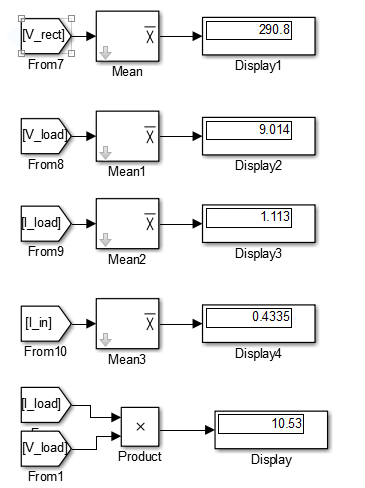
\includegraphics[width=8 cm]{VIvalues}
    \caption{All voltage current display values}
    \label{fig:display}
\end{figure}

Moreover, we have also checked that the switch voltage and current remains in the tolarable range. As expected, the voltage across the switch will be twice the input voltage when it turns off. This can be seen in figure\ref{fig:switch}.

\begin{figure}[H]
    \centering
    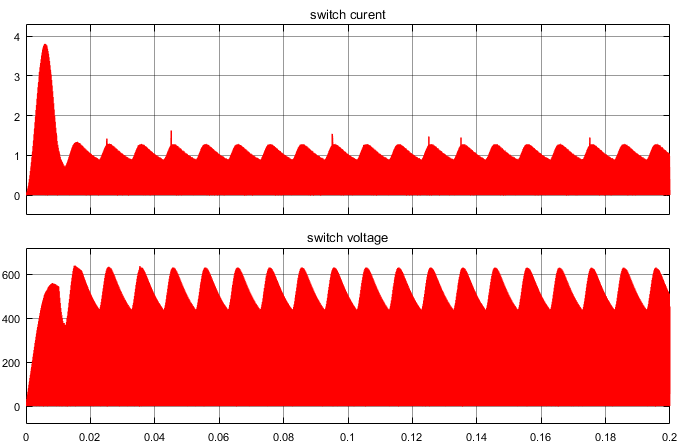
\includegraphics[width=15 cm]{switch_stress_snubbereffect}
    \caption{Current and voltage of the MOSFET during operation}
    \label{fig:switch}
\end{figure}

\subsection{Transformer Design}

For flyback topology design, there are many different considerations like loss, area, saturation etc. We started the topology knowing that the duty cycle can not exceed 0.5. Following the steps in \cite{cookcook}, we started by putting a safety margin to the duty cycle and selecting it to be 0.4. Once we have decided on this, using the flyback input output relation $N_{sec}/N{prim}\cdot D/(1-D) \cdot V_{in}=V_{out}$ ,since flyback is a buck boost topology, we found the turns ratio to be 19. Following this, we need the primary and secondary rms and average currents in order to decide on the core inductance and the exact turns ratio. We know that ideally we need around 1.2 A in secondary and .....

       
\section{Controller Design}

This part contains the desired control design for our flyback converter. The controller is chosen to be type 2 controller with a schematic shown in figure \ref{fig:controller}.
\begin{figure}[H]
    \centering
    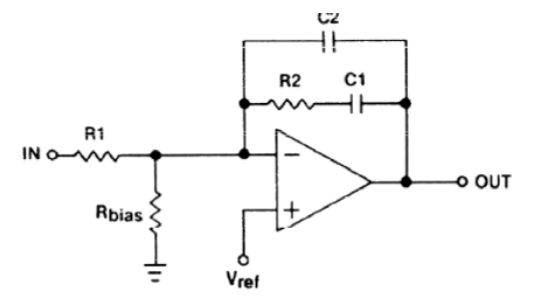
\includegraphics[width=15 cm]{controller}
    \caption{Type 2 Controller}
    \label{fig:controller}
\end{figure}

\subsection{Part 1. Controller Transfer Function}

The transfer function for the controller is:

\begin{equation*}
    \Tilde{v_{c}}/\Tilde{v_{o}}=Z_{feedback}/Z_{input}
\end{equation*}

COnsider that the input and output voltages contain DC and ACcomponents, while the reference is DC. In order to derive the transfer function, consider the AC components:


\begin{equation*}
    Z_{feedback}=1/sC_2// (R_2 +1/sC_1)\\
\end{equation*}
\begin{equation*}
Z_{input}=R_1 R_{bias}/(R_1 + R_{bias})
\end{equation*}

This yield the following transfer function:

\begin{equation*}
T_c(s)=\dfrac{R_1+R_{bias}}{R_1 R_{bias} }\cdot \dfrac{1}{C_2}\cdot \dfrac{s+1/(R_1 C_1)}{s(s+(C_1+C_2)/R_2C_1C_2)}
\end{equation*}

Here, we observe that the controller is a compensator function. It is in our control to make it either a lead or lag compensator. For stability, we need an increase in the phase margin of our close loop system. Hence, we desire the controller to add a phase lead (boost). Therefore, we need to place a zero before a pole so that first an incline in the phase occurs. The general bode plot for the controller transfer function is provided in figure \ref{fig:bode}, we see that the zero is placed before the pole. 

\begin{figure}[H]
    \centering
    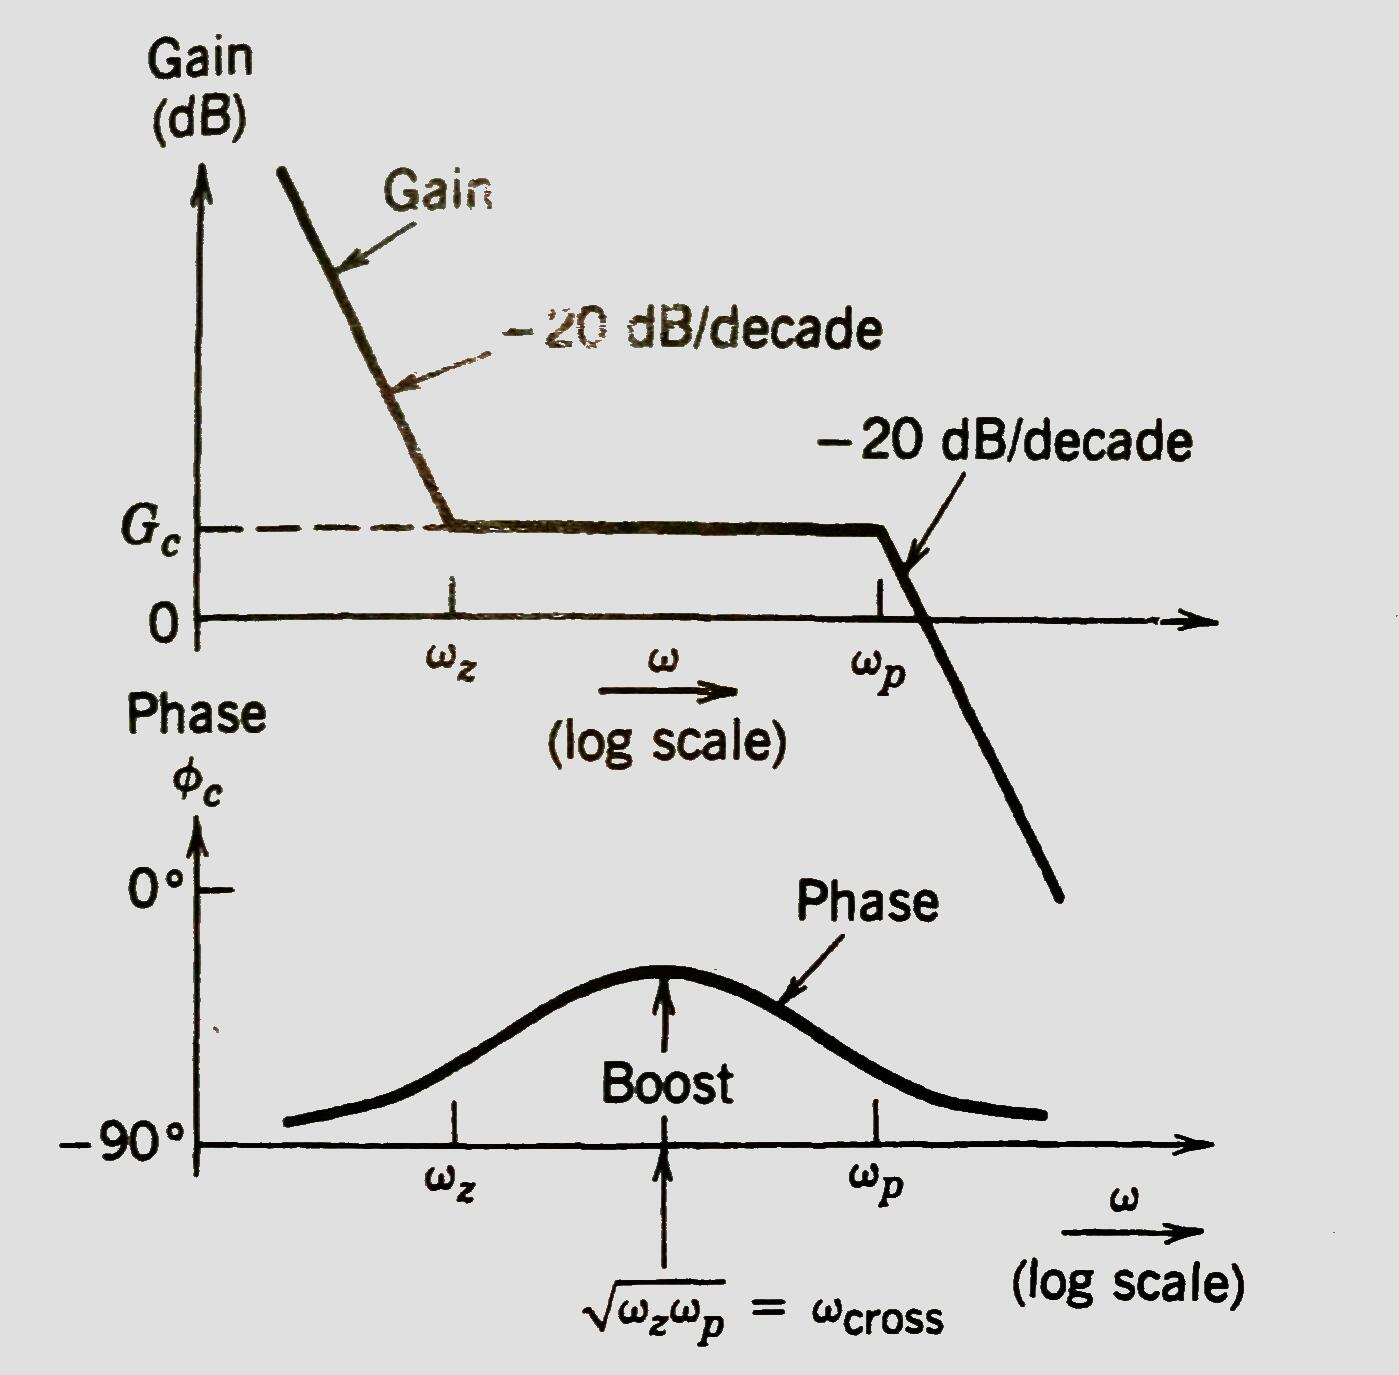
\includegraphics[width=10 cm]{bode}
    \caption{Type 2 Controller Bode Plot}
    \label{fig:bode}
\end{figure}

\subsection{Part 2. Controller Computer Simulation}


\end{document}
